\documentclass{beamer}

\beamertemplatenavigationsymbolsempty

\mode<presentation>
{
  \usetheme{default}
}

\usepackage[english]{babel}
\usepackage[latin1]{inputenc}
\usepackage{bussproofs}
\usepackage[retainorgcmds]{IEEEtrantools}

% needs debian package texlive-math-extra
\usepackage{stmaryrd} % for \llbracket, \rrbracket

\usepackage{times}
\usepackage[T1]{fontenc}
% Or whatever. Note that the encoding and the font should match. If T1
% does not look nice, try deleting the line with the fontenc.

\usepackage{tikz}
\usetikzlibrary{positioning}
\usetikzlibrary{calc}
\usetikzlibrary{matrix}
\usetikzlibrary{arrows}

\title
{Structural Subtyping for Records}

\author
{Markus~Klinik}

\institute[Radboud University Nijmegen]
{
  Radboud University Nijmegen
}

\date
{Compiler Construction 2013}


\newcommand{\arr}{\rightarrow}
\newcommand{\Arr}{\Rightarrow}
\newcommand{\semantics}[1]{\llbracket #1 \rrbracket}
\newcommand{\semanticsFd}[1]{\semantics{#1}_{F\delta}}
\newcommand{\oftype}[2]{#1\!:\!#2}

\begin{document}

\begin{frame}
  \titlepage
\end{frame}

\begin{frame}[fragile]{We've All Been There}

\begin{verbatim}
def printXY(a):
  print a.x
  print a.y

class X:
  x = 10

printXY(X())
\end{verbatim}

\end{frame}

\begin{frame}[fragile]{That's What They Want}

\begin{verbatim}
class XY:
  x = []
  y = False

class XYZ:
  x = "Elvis lives"
  y = True
  z = 10

printXY(XY())
printXY(XYZ())
\end{verbatim}

\end{frame}


\begin{frame}{What Is a Record?}

\begin{itemize}
  \item What do we want to do with a record?
  \item Introduction and elimination!
\end{itemize}

\end{frame}


\begin{frame}[fragile]{Introduction And Elimination}

\onslide<+->

Introduction

\begin{verbatim}
var rec = { x=10, y=True }
printXY( { x=10, z=[] } )
\end{verbatim}

\onslide<+->

Elimination

\begin{verbatim}
rec.x
\end{verbatim}

\end{frame}


\begin{frame}[fragile]{But What \emph{is} a Record?}

\onslide<+->

\begin{itemize}
  \item How is it stored in memory?
  \item How does the code for record projection look like?
\end{itemize}

\onslide<+->

The code

\begin{verbatim}
a getX({a x} b) { return b.x; }
\end{verbatim}

must work for:

\begin{verbatim}
getX({x=10})
getX({y=True,x=False})
\end{verbatim}

and any other combination of fields.

\end{frame}


\begin{frame}[fragile]{Records Are Association Lists}

\texttt{\{ x=10, y=True \}}

\vspace{3em}

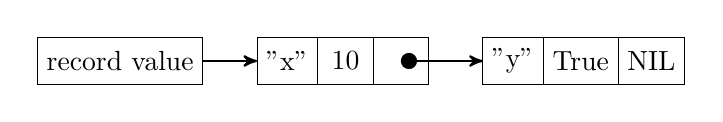
\begin{tikzpicture}

  \matrix [matrix of nodes
    , nodes={ minimum height = 1.7em
            , minimum width = 2em
            , outer sep = 0pt
            , anchor = north
            }
    , column sep=-\pgflinewidth % collapse borders
    , nodes in empty cells]
  {
    |(record)[draw]|record value & &
      |(x)[draw]|"x" & |(ten) [draw]|10   & |(xnext)[draw]| & &
      |(y)[draw]|"y" & |(true)[draw]|True & |(ynext)[draw]|NIL \\
  };

  \draw [-stealth', thick] (record.east) to (x.west);
  \draw [*-stealth', thick] (xnext.center) to (y.west);

\end{tikzpicture}

\end{frame}

\begin{frame}[fragile]{Well, More Like Association Arrays}

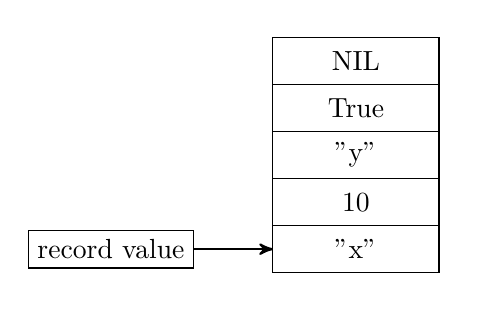
\begin{tikzpicture}

  \matrix (record) [matrix of nodes
    , nodes={ minimum height = 1.7em
            , minimum width = 6em
            , outer sep = 0pt
            , anchor = north
            , draw
            }
    , column sep=-\pgflinewidth % collapse borders
    , row sep=-\pgflinewidth % collapse borders
    , nodes in empty cells]
  {
    NIL   \\
    True  \\
    "y"   \\
    10    \\
    |(x)| "x" \\
  };

  \node (value) [left = of x,draw] {record value};

  \draw [-stealth',thick] (value.east) to [out=0,in=180] (x.west);

\end{tikzpicture}

\end{frame}


\begin{frame}{Type Checking For Records}
\begin{itemize}
  \item Type inference
  \item Subtyping
  \item Mitchell Wand, 1987, Complete Type Inference for Simple Objects
\end{itemize}
\end{frame}

\begin{frame}{Subtyping}
\begin{itemize}
  \item $\alpha$ is a subtype of $\beta$
  \item $\alpha <: \beta$
  \item $\alpha$ can be used when $\beta$ is expected
  \item $\alpha$ has \emph{more} fields than $\beta$
\end{itemize}
\end{frame}

\begin{frame}{Subtyping and Lists}
\begin{itemize}%[<+->]
  \item If $\alpha <: \beta$ then $[\alpha] <: [\beta]$
  \item Lists are \emph{covariant}
  \item Lists are uniform
  \item Tuples and return types of functions are also covariant
\end{itemize}
\end{frame}

\begin{frame}[fragile]{Subtyping and Higher-Order Functions}

\onslide<+->
\begin{itemize}
  \item Function argument types are \emph{contravariant}
  \item If $\beta <: \alpha$ then $\alpha \arr \tau <: \beta \arr \tau$
\end{itemize}

\onslide<+->

Example

\begin{verbatim}
Int H( ({Int x, Int y} -> Int) f )
{
  return f( { x=10, y=20 } );
}
\end{verbatim}

\begin{itemize}
  \item $\text{foo} : (\{\text{Int}\ x\} \arr \text{Int})$
  \item $\text{bar} : (\{\text{Int}\ x, \text{Int}\ y, \text{Int}\ z\} \arr \text{Int})$
\end{itemize}

\end{frame}


\begin{frame}{Type Inference For Records}

\onslide<+->

Milner's Idea:

\begin{enumerate}
  \item Take all type variables from a derivation
  \item Make a set of \emph{constraints}
  \item Run Robinson's unification algorithm on the constraints
\end{enumerate}

\onslide<+->

Wand's Idea:

\begin{enumerate}
  \item Make a system of \emph{rows} with variables
  \item Step 2 and 3 as above
\end{enumerate}

\end{frame}


\begin{frame}{What Is a Row?}

\begin{itemize}
  \item A row is either empty,
  \item Or a set of name/type pairs extending some other row
  \item Rows give rise to record types
\end{itemize}

Example

\begin{equation*}
  \rho[\oftype{x}{\text{Int}}, \oftype{y}{\text{Bool}}]
\end{equation*}

\end{frame}


\begin{frame}{Example}

\texttt{f( \{ x=10, y=True \} )}
\vspace{1em}

Given the constraint

\begin{IEEEeqnarray*}{rCl}
\sigma[\oftype{x}{\text{Int}}] & = & \rho[\oftype{x}{\text{Int}}, \oftype{y}{\text{Bool}}]
\end{IEEEeqnarray*}

we know that:
\begin{IEEEeqnarray*}{rCl}
  \sigma & = & \tau[\oftype{y}{\text{Bool}}] \\
  \rho & = & \tau
\end{IEEEeqnarray*}

so:
\begin{IEEEeqnarray*}{rCl}
  \tau[\oftype{y}{\text{Bool}}][\oftype{x}{\text{Int}}] & = &
    \tau[\oftype{x}{\text{Int}}, \oftype{y}{\text{Bool}}]
\end{IEEEeqnarray*}


\end{frame}


\begin{frame}{Demo}
\end{frame}


\end{document}
